\documentclass[12pt]{article}

\pdfoutput=24
\usepackage{amsmath}
\usepackage{amsthm}
\usepackage{esvect}
\usepackage[toc,page]{appendix}
\usepackage{leftidx}
\usepackage{color}
\usepackage{framed, color}
\usepackage{multirow}
\usepackage{pdfpages}
\usepackage{multicol}
\usepackage{wrapfig,lipsum,booktabs}

\usepackage[utf8]{inputenc}
\usepackage{mathtools,hyperref}
\hypersetup{
    colorlinks=true,
    linkcolor=cyan,
    filecolor=cyan,      
    urlcolor=red,
    citecolor=red,
}

\def\code#1{\textbf{\texttt{#1}}}
\def\vari#1{{\color{Cerulean}{\textbf{\texttt{#1}}}}}
\def\func#1{{\color{Maroon}{\textbf{\texttt{#1}}}}}
\newenvironment{coded}{\color{blue}\code}


\usepackage{cleveref}
\usepackage{commath}
\usepackage{enumitem}
\usepackage{amssymb}
\renewcommand{\qedsymbol}{$\blacksquare$}

%%%%%%%%%%%
%%%%%%%%%%%  User Defined Commands. (macros)
%%%%%%%%%%%

\definecolor{mgreen}{RGB}{25,147,100}
\definecolor{shadecolor}{rgb}{1,.8,.1}
\definecolor{shadecolor2}{RGB}{245,237,0}
\definecolor{orange}{RGB}{255,137,20}
\definecolor{orange}{RGB}{245,37,100}

%%%%%%%%%%%
%%%%%%%%%%%  Graphical Packages
%%%%%%%%%%%
\usepackage{pgfplots}
\usetikzlibrary{patterns}
\usepackage{mdframed}
\usepackage{adjustbox}
\usepackage{tcolorbox}
%\usepackage{graphics}
\usepackage{tikz,ifthen,fp,calc}
\usepackage{caption}
\usepackage{subcaption}
\usetikzlibrary{plotmarks}
\usepackage{graphicx}

%%%%%%%%%%%%%%%%%
%%%%%%%%%%%%%%%%% Theorem Styles
%%%%%%%%%%%%%%%%%
\theoremstyle{plain}
\newtheorem{theorem}{Theorem}[section]
\newtheorem{prop}{Proposition}[section]
\newtheorem{corr}{Corollary}[section]
\theoremstyle{definition}
\newtheorem{definition}{Definition}[section]
\newtheorem{lemma}[theorem]{Lemma}
\theoremstyle{definition}
\newtheorem{remark}{Remark}[section]
\newtheorem{fact}{Fact}[section]

\usepackage[english]{babel}
\usepackage{babel,blindtext}
\newtheorem{corollary}{Corollary}[theorem]
\newtheorem{exmp}{Example}[section]
\usepackage{fullpage}
\usepackage{amsfonts}
\usepackage{lscape}
\usepackage{bbm}

\usepackage{todonotes}
\usepackage{cite}
\usepackage{verbatim}
\usepackage{bm}

\DeclareMathOperator*{\argmax}{arg\,max}
\usepackage[margin=1in]{geometry}
\providecommand{\keywords}[1]{\textbf{\textit{Keywords:---}} #1}

\usepackage[T1]{fontenc}
\usepackage[utf8]{inputenc}
\usepackage{authblk}
\usepackage{cite}


\newcommand*{\affaddr}[1]{#1} % No op here. Customize it for different styles.
\newcommand*{\affmark}[1][*]{\textsuperscript{#1}}
%\newcommand*{\email}[1]{\texttt{#1}}

\date{}

\providecommand{\keywords}[1]{\textbf{\textit{Keywords:}} #1}

\begin{document} 

Let $\lambda$ be the scale, $\kappa$ be the shape factors of
the Weibull distribution. Then the variance is given by

\begin{equation}
  \label{eq:variance}
\sigma = \lambda^2 [\Gamma(1 + 2/\kappa) - (\Gamma(1+1/\kappa))^2]
\end{equation}


Equation~\eqref{eq:variance} on its own shows increase 
of $\lambda$ increase in the variance (when $\lambda > 1$).

For the original model, the parameters of larva generation 1 is given by:

\[(\kappa, \lambda) = (4.42486, \:742.9410)\]

If we increase the scale by 10\% and 20\%
we get 
\[(\kappa_{10}, \lambda_{10}) = (4.42486,\: 817.2351)\] 
and 
\[(\kappa_{20}, \lambda_{20}) = (4.42486, \: 891.5292)\]
 respectively. Computing the variance then would be easy.

\iffalse

For generation 4 of larva we have

\[(\kappa, \lambda) = (16.080100, \: 4065.2020)\]
\[(\kappa_{10}, \lambda_{10}) = (16.080100, \: 4471.7222)\]
\[(\kappa_{20}, \lambda_{20}) = (16.080100, \: 4878.2424)\]


If we draw a line at $y = 0.0005$ in the Weibull distribution 
plot, and we compute the length of the section cutting the
Weibull distribution we get $$
 \fi

\begin{figure}[httb!]
  \centering
  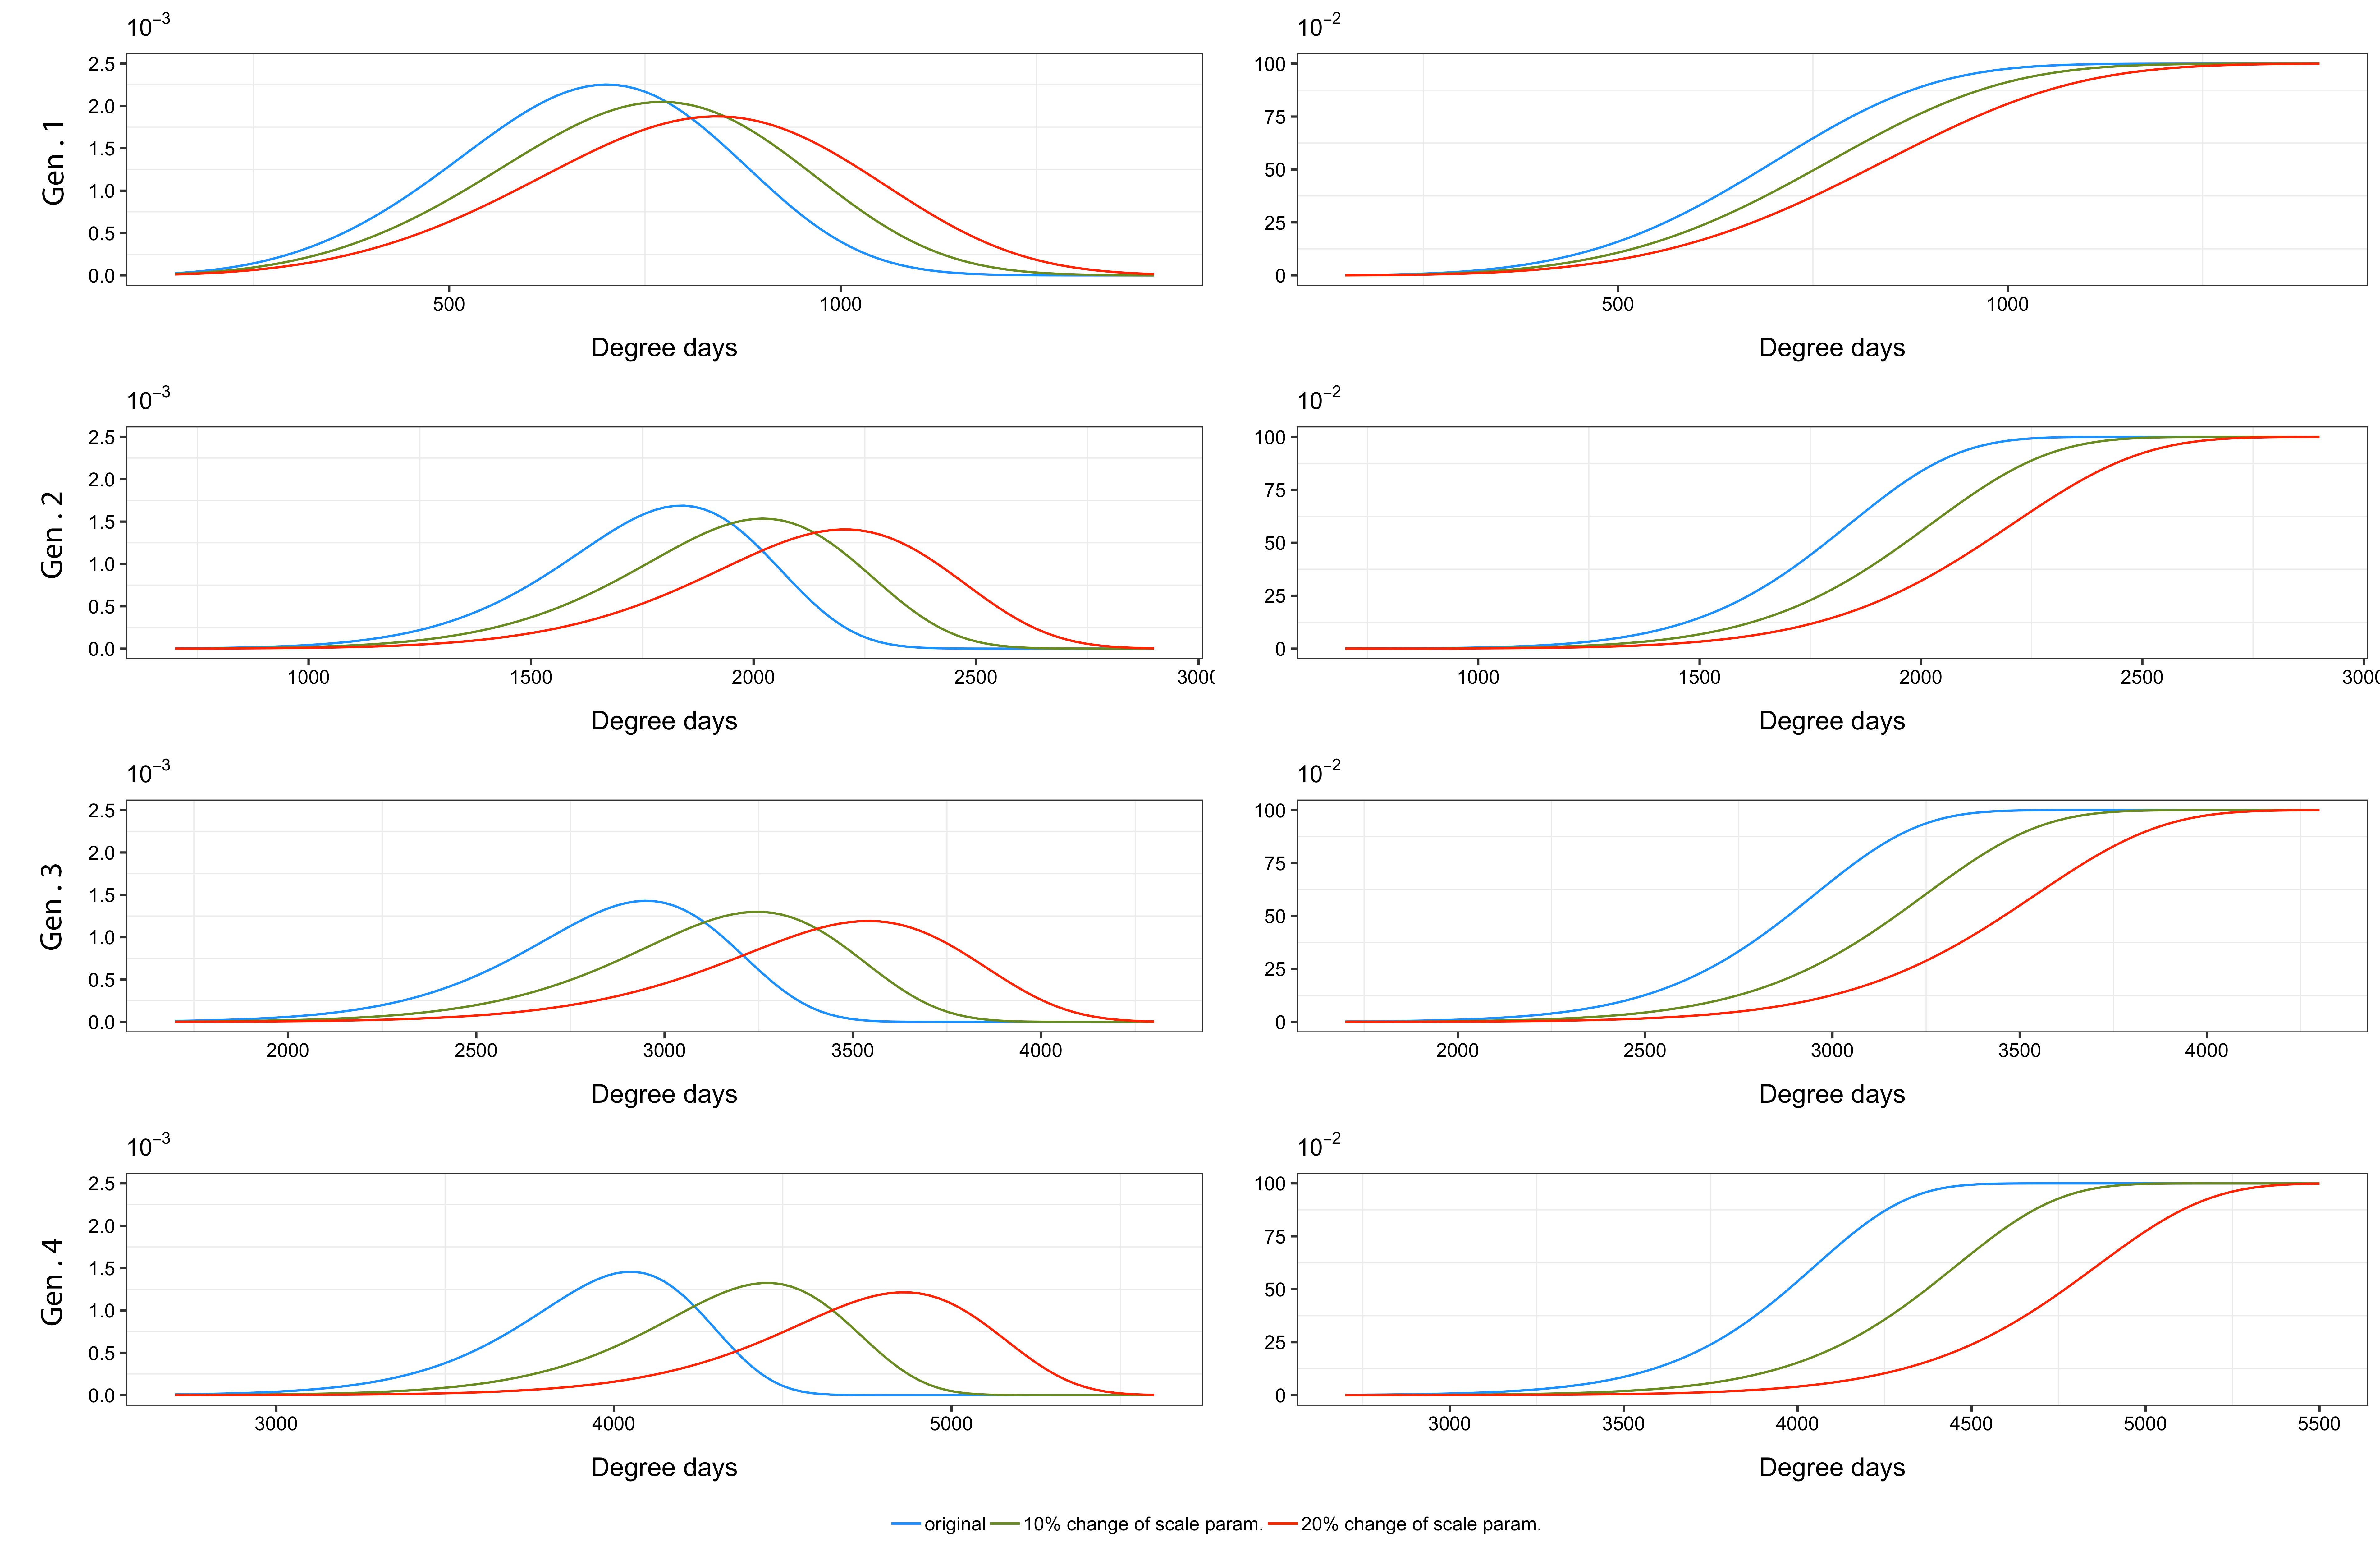
\includegraphics[width=1\linewidth]{larva_weibull.png}
\caption{Weibull density and cumulitive distributions.}
\label{fig:degrootevolution}
\end{figure}

Also, the lowered peaks show, the distributions are not 
just shifted.

\section{Another take from cumulative function}
The cumulative function of Weibull is given by
\[ f(x, \lambda, \kappa) = 1- exp(-(x/\lambda)^\kappa)\]

hence, 
\[ f'(x, \lambda, \kappa) = \kappa/\lambda (x/\kappa)^{\kappa-1} - exp(-(x/\lambda)^\kappa) \]

Using R and quantile function we can find the $x$'s for which cumulative probability is $0.5$.

\code{ qweibull(0.5, shape=shape, scale=scale\_orig)} produces $x = 683.8826$.

\code{ qweibull(0.5, shape=shape, scale=scale\_10\_percent)} produces $x_{10} = 752.2708$.

\code{ qweibull(0.5, shape=shape, scale=scale\_20\_percent)} produces $x_{20} = 820.6591$.\\

Plugging the shape and scales with associated $x$ into the derivative equation above we get



\begin{equation}
\left\{
  \begin{array}{lr}
    f'(x, \lambda, \kappa\_{orig})  &= 0.002242402 \vspace{.1in}\\
    f'(x_{10}, \lambda, \kappa_{\_10\_percent}) &= 0.002038547 \vspace{.1in}\\
    f'(x_{20}, \lambda, \kappa_{\_20\_percent}) &= 0.001868668
    
  \end{array}
\right.
\end{equation}

Though, they are close, and visually may seem shifted, they are not.

\end{document}
